\documentclass[10pt,a4paper]{article}

% Layout
\usepackage[margin=0.8in]{geometry}
\usepackage{fancyhdr}
\usepackage{titlesec}
\usepackage{enumitem}
\usepackage{float}

% Math / Tables
\usepackage{amsmath,amsfonts}
\usepackage{booktabs}

% Graphics / Plots
\usepackage{tikz}
\usepackage{pgfplots}
\pgfplotsset{compat=1.18}

% Fonts / Colors / Links
\usepackage{lmodern}
\renewcommand{\familydefault}{\sfdefault}
\usepackage{xcolor}
\usepackage{hyperref}
\usepackage{tocloft}

% Code listings
\usepackage{listings}

% ---------- Reusable variables ----------
\newcommand{\NoteTitle}{Time Series Analysis}
\newcommand{\NoteAuthor}{Thomaskutty Reji}

% ---------- Spacing ----------
\setlength{\parskip}{2.5pt}
\setlength{\parindent}{0pt}
\setlength{\headheight}{14pt}
\setlength{\abovedisplayskip}{5pt}
\setlength{\belowdisplayskip}{5pt}
\setlength{\abovedisplayshortskip}{3pt}
\setlength{\belowdisplayshortskip}{3pt}
\setcounter{secnumdepth}{3}

\setlist[itemize]{leftmargin=1.8em,labelwidth=0.8em,labelsep=0.35em,itemsep=2pt,topsep=2pt,parsep=0pt,partopsep=0pt}
\setlist[enumerate]{leftmargin=2.0em,labelsep=0.4em,itemsep=2pt,topsep=2pt,parsep=0pt,partopsep=0pt}

% ---------- Colors ----------
\definecolor{tocblue}{HTML}{0345fc}
\colorlet{accent}{tocblue}

\definecolor{softgreen}{HTML}{E6F4EA}
\definecolor{softyellow}{HTML}{FFF6D6}
\definecolor{softblue}{HTML}{D6E7F8}

\definecolor{codebg}{RGB}{245,245,245}
\definecolor{codeblue}{RGB}{0,70,180}
\definecolor{codecomment}{RGB}{90,90,90}
\definecolor{codestring}{RGB}{160,60,0}

% ---------- Section styles ----------
\titleformat{\section}{\LARGE\color{accent}}{\thesection}{0.8em}{}
\titleformat{\subsection}{\Large\color{accent}}{\thesubsection}{0.8em}{}
\titleformat{\subsubsection}{\large\color{accent}}{\thesubsubsection}{0.8em}{}
\titlespacing*{\section}{0pt}{9pt}{4pt}
\titlespacing*{\subsection}{0pt}{7pt}{3pt}
\titlespacing*{\subsubsection}{0pt}{6pt}{2pt}

% ---------- TOC styles ----------
\renewcommand{\cftsecfont}{\color{tocblue}}
\renewcommand{\cftsubsecfont}{\color{tocblue}}
\renewcommand{\cftsubsubsecfont}{\color{tocblue}}
\renewcommand{\cftsecpagefont}{\color{tocblue}}
\renewcommand{\cftsubsecpagefont}{\color{tocblue}}
\renewcommand{\cftsubsubsecpagefont}{\color{tocblue}}
\setlength{\cftbeforesecskip}{0pt}

% ---------- Header / Footer ----------
\pagestyle{fancy}
\fancyhf{}
\fancyhead[L]{\NoteTitle}
\fancyhead[R]{\textbf{}}
\fancyfoot[L]{\hyperref[toc]{Table of Contents}}
\fancyfoot[R]{\thepage}
\renewcommand{\headrulewidth}{0.4pt}
\renewcommand{\footrulewidth}{0.4pt}

\fancypagestyle{plain}{
  \fancyhf{}
  \fancyhead[L]{\NoteTitle}
  \fancyhead[R]{\textbf{}}
  \fancyfoot[L]{\hyperref[toc]{Table of Contents}}
  \fancyfoot[R]{\thepage}
  \renewcommand{\headrulewidth}{0.4pt}
  \renewcommand{\footrulewidth}{0.4pt}
}

% ---------- Custom commands ----------
\newcommand{\Set}[1]{\left\{#1\right\}}

% ---------- Listings ----------
\lstdefinestyle{github}{
  language=Python,
  backgroundcolor=\color{codebg},
  basicstyle=\ttfamily\small,
  keywordstyle=\color{codeblue}\bfseries,
  identifierstyle=\color{black},
  commentstyle=\color{codecomment}\itshape,
  stringstyle=\color{codestring},
  showstringspaces=false,
  frame=single,
  rulecolor=\color{black!20},
  breaklines=true,
  tabsize=4
}

\lstset{
  language=Python,
  basicstyle=\ttfamily\small,
  keywordstyle=\color{blue},
  commentstyle=\color{gray},
  stringstyle=\color{orange},
  showstringspaces=false,
  frame=single,
  breaklines=true
}

% ---------- Hyperlinks ----------
\hypersetup{
  colorlinks=true,
  linkcolor=tocblue,
  citecolor=tocblue,
  urlcolor=tocblue
}

\begin{document}

\begin{titlepage}
  \vspace*{0.25\textheight}
  {\LARGE \textcolor{tocblue}{\NoteTitle}}\par
  \author{\NoteAuthor}
  \date{}
\end{titlepage}

\phantomsection
\label{toc}
\tableofcontents
\newpage
\section{Time Series Analysis}
	\subsection{Time Series Components}
	$$
	X_t (\text{Observed}) = \text{Trend} + \text{Seasonality} + \text{Cyclic} + \text{Irregular}
	$$
	
	
	\begin{itemize} 
	    \item Trend captures the overall direction(up, down , flat)
	    \item Seasonality refers to the repeating pattern at a fixed frequency ( quarterly, monthly, daily)
	    \item Cyclic component refers to the long term oscillations. It can be a business cycle, economic booms, recessions etc.
	    \item Irregular Noise : random fluctuations, unpredictable shocks. Often modeled as white noise.
	\end{itemize}
	
	\subsection{Additive vs Multiplicative Decompositions}
	
	\begin{itemize}
	    \item We use additive decomposition of the series when seasonal variation is constant over time. We use multiplicative decomposition when seasonal fluctuations grow with level. 
	\end{itemize}
	
	
	\subsection{Mean Absolute Percentage Error (MAPE)}
	Measures the average absolute percentage difference between actual values $A_t$ and forecasted values $F_t$:
	
	\[
	\text{MAPE} = \frac{100\%}{n} \sum_{t=1}^{n} \left| \frac{A_t - F_t}{A_t} \right|
	\]
	
	\begin{itemize}
	    \item Range: $[0\%, \infty)$ (undefined if any $A_t = 0$)
	    \item Interpretation: Lower MAPE indicates more accurate forecasts.
	    \item Limitation: Sensitive to zeros and very small actual values.
	\end{itemize}
	
	\subsection{Symmetric Mean Absolute Percentage Error (sMAPE)} 
	Adjusts for zeros and small values by normalizing the error with the average of actual and forecast:
	
	\[
	\text{sMAPE} = \frac{100\%}{n} \sum_{t=1}^{n} \frac{|F_t - A_t|}{(|A_t| + |F_t|)/2}
	\]
	
	\begin{itemize}
	    \item Range: $[0\%, 200\%]$
	    \item Interpretation: Lower sMAPE indicates better forecasts; symmetric treatment avoids extreme percentages.
	    \item Advantage: Handles zeros and small values gracefully.
	\end{itemize}
	
	
	
	\subsection{Deterministic vs Stochastic Models}
	\begin{itemize}
	    \item \textbf{Deterministic} : Once the parameters are fixed, the forecast is completely determined by past observations \& No explicit modeling of randomness.
	    \item \textbf{Stochastic}: The data generating process explicitly includes a random error term. Forecasts are distributions, not just point values.
	\end{itemize}
	
	\subsection{Stationary Series}
	
	%\begin{conceptbox}
	A time series is \textbf{stationary} if its statistical properties remain constant over time.
	%\end{conceptbox}
	
	A stationary series satisfies:
	
	
	\begin{itemize}
	\item Mean is constant
	\item Variance is constant
	\item Autocovariance depends only on the lag
	\end{itemize}
	
	
	Most classical time series models such as \textbf{ARIMA} assume weak stationarity.
	
	
	\textbf{Weak Stationarity}
	
	Only the first two moments are constant:
	\begin{align*}
	E[X_t] = \mu \\
	Var(X_t) = \sigma^2
	\end{align*}
	
	
	
	\textbf{Strong Stationarity}
	\begin{align*}
	(X_{t_1}, X_{t_2}, ..., X_{t_k})
	\overset{d}{=}
	(X_{t_1+h}, X_{t_2+h}, ..., X_{t_k+h})
	\end{align*}
	
	The entire probability distribution is unchanged over time.
	
	\subsection{Augmented Dickey-Fuller Test : Stationarity}
	
	A central concept in time series analysis is \textit{stationarity}, which informally means that the statistical properties of a process (such as mean and variance) do not change over time. Many econometric and statistical methods rely on this assumption. A key source of non-stationarity is the presence of a \textit{unit root}.
	
	Consider the first-order autoregressive process:
	\begin{align*}
	X_t = \phi X_{t-1} + \epsilon_t,
	\end{align*}
	where $\epsilon_t$ is white noise. The behavior of the process depends critically on the value of $\phi$:
	\begin{itemize}
	\item If $|\phi| < 1$, the process is stationary and mean-reverting.
	\item If $\phi = 1$, the process becomes a \textit{random walk}:
	\begin{align*}
	X_t = X_{t-1} + \epsilon_t,
	\end{align*}
	in which shocks accumulate permanently, leading to non-stationarity.
	\end{itemize}
	
	The case $\phi = 1$ is referred to as a \textit{unit root}. The term arises from the characteristic equation of the lag operator representation, where a root equal to one implies non-stationarity. Intuitively, a unit root indicates that shocks have persistent effects and the series does not revert to a long-run mean.
	
	To test for a unit root, we rewrite the model by subtracting $X_{t-1}$ from both sides:
	\begin{align*}
	\Delta X_t &= X_t - X_{t-1} \\
	&= (\phi - 1) X_{t-1} + \epsilon_t \\
	&= \delta X_{t-1} + \epsilon_t,
	\end{align*} 
	where $\delta = \phi - 1$. The testing problem becomes:
	\begin{align*}
	H_0 &: \delta = 0 \quad (\text{unit root, non-stationary}) \\
	H_1 &: \delta < 0 \quad (\text{stationary})
	\end{align*}
	
	This forms the basis of the \textit{Dickey--Fuller (DF) test}. Rejection of the null hypothesis suggests that the series is stationary. The test uses non-standard critical values due to the non-standard distribution of the estimator under the null.
	
	The basic DF test relies on the assumption that the error term $\epsilon_t$ is uncorrelated. However, in practical applications, time series often exhibit higher-order serial correlation. To account for this, the model is extended by including lagged differences of the dependent variable:
	\begin{align*}
	\Delta X_t = \delta X_{t-1} + \sum_{i=1}^{p} \gamma_i \Delta X_{t-i} + \epsilon_t.
	\end{align*}
	
	This specification is known as the \textit{Augmented Dickey--Fuller (ADF) test}. The additional lagged difference terms capture short-run dynamics and ensure that the error term is approximately white noise. The hypothesis being tested remains unchanged:
	\begin{align*}
	H_0 &: \delta = 0 \quad (\text{unit root}) \\
	H_1 &: \delta < 0 \quad (\text{stationary})
	\end{align*}
	
	The inclusion of lagged differences does not alter the fundamental objective of the test; rather, it improves its validity in the presence of autocorrelated errors. The number of lags $p$ is typically selected using information criteria such as AIC or BIC.
	
	In summary, the Dickey--Fuller framework provides a formal mechanism to detect whether a time series exhibits a unit root, i.e., whether shocks have permanent effects. The augmented version generalizes this approach to more realistic settings by allowing for richer temporal dependence.
	
	
	
	\subsection{Box-Cox Transformation}
	
	The Box-Cox transformation generalizes the log transformation by searching across a family of power transformations.
	
	
	\[
	\begin{cases}
	\dfrac{X_t^{\lambda} - 1}{\lambda}, & \lambda \neq 0 \\
	\log(X_t), & \lambda = 0
	\end{cases}
	\]
	
	\begin{itemize}
	\item Smaller $\lambda$ values compress large observations more strongly.
	\item The transformation is chosen so that the transformed data has approximately constant variance and resembles Gaussian white noise.
	\end{itemize}
	
	
	\subsection{Backshift Operator \& Differencing}
	The backshift operator B shifts a time series back by one time period. 
	$$
	B X_t = X_{t-1}
	$$
	$$
	B^k X_t = X_{t-k}
	$$
	First order Differencing : removes the linear trend. This is the most common differencing used in ARIMA (d=1). Measures the change in level. $\Delta X_t = X_t - X_{t-1}$. 
	
	Using the backshift operator ; $\Delta X_t = (1 - B) X_t$
	
	Second order differencing: $\Delta^2 X_t = \Delta(\Delta X_t)$
	
	Simplified Form : $\Delta^2 X_t = X_t - 2X_{t-1} + X_{t-2}$
	
	Using the backshift Operator : $\Delta^2 X_t = (1 - B)^2 X_t$
	
	General Differencing Term : $\Delta^d X_t = (1 - B)^d X_t$
	
	When we apply differencing on a series like 101,104, 112,… like this (example) . The absolute baseline value is gone. Only changes remain. This is why the differenced series oscillates around zero. 
	
	\subsection{Trend of a Time Series}
	\begin{itemize}
	    \item Trend is the systematic, long-term movement of the level over time. It answers : Is the baseline drifting up, down, or staying flat?
	    \item In a linear model : $X_t = a + bt + \epsilon_t$; a is the baseline. b is trend( average change per time unit) and epsilon is the noise.
	    \item But trend can also be piecewise, nonlinear, stochastic ( random walk with drift)
	    \item \textbf{Deterministic Trend}  : The trend is fixed and predictable, like a straight line ( or a polynomial). Differencing removes this trend, but you could also remove it by regression de-trending.
	    \item \textbf{Stochastic Trend}: The trend is random and cumulative - it depends on past shocks. Random walk with drift  $X_t = X_{t-1} + c + \epsilon_t$. Trend is accumulated random shocks, slope is not fixed. Most economic time series have stochastic trends.
	\end{itemize}
	
	\subsection{White Noise}
	A special case of a stationary series with the following properties;
	
	\begin{itemize}
	    \item Mean = 0 ( or constant )
	    \item Variance = constant over time
	    \item No autocorrelation:  $Cov(X_t,X_{t-k}) = 0 ; \forall k \neq 0 $
	\end{itemize}
	
	Every observation is completely random, independent of past values. No memory → Unpredictable. Examples are random shocks, coin flips, Gaussian noise. White noise is stationary ( means and variance constant), but it is not predictable because past values give no information about future values.
	
	
	
	\subsection{Forecasting Methods}
	\begin{itemize}
	    \item \textbf{Expanding Forecast} : Model is trained on an increasing window of data, includes all past observations up to current point. - Computationally expensive, History is important
	    \item \textbf{Rolling Forecast} : Recursive, actual value from the previous period is used for next prediction.
	    \item \textbf{Simple Moving Average} : Average of fixed number of past observations. Each observation is given equal weight
	    \item \textbf{Weighted Moving Average} : Giving more importance to recent values.
	\end{itemize}
	
	\subsection{Simple Exponential Smoothing}
	
	Simple Exponential Smoothing (SES) is suitable for time series data with \textbf{no clear trend or seasonality}. It updates the forecast by combining the latest observation with the previous forecast.
	
	\begin{align*}
	\large \hat{y}_{t+1} = \alpha y_t + (1-\alpha)\hat{y}_t
	\end{align*}
	
	where:
	\begin{itemize}
	\item $\alpha$ is the smoothing parameter ($0 < \alpha < 1$)
	\item $y_t$ is the observed value at time $t$
	\item $\hat{y}_t$ is the forecast at time $t$
	\end{itemize}
	
	This method works well for \textbf{stationary time series} and is generally used for \textbf{short-term forecasting}.
	
	\medskip
	
	\textbf{Example} Suppose $\alpha = 0.3$ and the observed series is: [50,52,49,53]
	
	\begin{center}
	\begin{tabular}{c|c|c|c}
	\hline
	$t$ & $y_t$ & $\hat{y}_t$ & $\hat{y}_{t+1} = \alpha y_t + (1-\alpha)\hat{y}_t$ \\
	\hline
	1 & 50 & 50.00 & $0.3(50) + 0.7(50) = 50.00$ \\
	2 & 52 & 50.00 & $0.3(52) + 0.7(50) = 50.60$ \\
	3 & 49 & 50.60 & $0.3(49) + 0.7(50.60) = 50.12$ \\
	4 & 53 & 50.12 & $0.3(53) + 0.7(50.12) = 50.98$ \\
	\hline
	\end{tabular}
	\end{center}
	
	\medskip
	
	\textbf{Interpretation.}
	\begin{itemize}
	\item Each new forecast is a weighted average of the current observation and the previous forecast.
	\item Recent observations get weight $\alpha$, while past information is retained through $(1-\alpha)$.
	\item Smaller $\alpha$ leads to smoother forecasts (slow reaction), while larger $\alpha$ reacts quickly to changes.
	\end{itemize}
	
	
	\subsection{Holt's Linear Trend Method}
	
	Simple Exponential Smoothing assumes no trend. If the time series contains a \textbf{trend}, Holt's method extends SES by introducing a trend component.
	
	\textbf{Level ($L_t$)}: Represents the current value of the series after adjusting for trend.
	
	\textbf{Trend ($T_t$)}: Represents the average change per period (slope of the series).
	
	\[
	L_t = \alpha X_t + (1 - \alpha)(L_{t-1} + T_{t-1}) \\
	T_t = \beta (L_t - L_{t-1}) + (1 - \beta)T_{t-1} \\
	\hat{X}_{t+h} = L_t + hT_t
	\]
	
	where:
	\begin{itemize}
	\item $L_t$ is the level component
	\item $T_t$ is the trend component
	\item $\alpha$ is the level smoothing parameter
	\item $\beta$ is the trend smoothing parameter
	\item $h$ is the forecast horizon
	\end{itemize}
	
	\medskip
	
	\textbf{Example.} Suppose $\alpha = 0.3$, $\beta = 0.2$, and the observed series is:
	\[
	[50, 52, 49, 53, 55, 54]
	\]
	
	Initialize:
	\[
	L_1 = y_1 = 50, \quad T_1 = y_2 - y_1 = 2.
	\]
	
	\medskip
	
	\begin{center}
	\begin{tabular}{c|c|c|c|c}
	\hline
	$t$ & $y_t$ & $L_t$ & $T_t$ & $\hat{y}_{t+1} = L_t + T_t$ \\
	\hline
	1 & 50 & 50.00 & 2.00 & 52.00 \\
	2 & 52 & $0.3(52) + 0.7(50+2) = 52.00$ & $0.2(52-50) + 0.8(2) = 2.00$ & 54.00 \\
	3 & 49 & $0.3(49) + 0.7(52+2) = 52.50$ & $0.2(52.5-52) + 0.8(2) = 1.70$ & 54.20 \\
	4 & 53 & $0.3(53) + 0.7(52.5+1.7) = 53.34$ & $0.2(53.34-52.5) + 0.8(1.7) = 1.53$ & 54.87 \\
	5 & 55 & $0.3(55) + 0.7(53.34+1.53) = 54.41$ & $0.2(54.41-53.34) + 0.8(1.53) = 1.44$ & 55.85 \\
	6 & 54 & $0.3(54) + 0.7(54.41+1.44) = 55.10$ & $0.2(55.10-54.41) + 0.8(1.44) = 1.29$ & 56.39 \\
	\hline
	\end{tabular}
	\end{center}
	
	\medskip
	
	\textbf{Interpretation.}
	\begin{itemize}
	\item The level $L_t$ follows the data while adjusting for the existing trend.
	\item The trend $T_t$ gradually adapts as the slope of the series changes.
	\item Forecasts extend the series linearly using the latest level and trend.
	\item With more data points, the smoothing behavior becomes clearer and more stable.
	\end{itemize}
	
	
	\subsection{Holt-Winters Seasonal Model}
	
	The Holt-Winters method extends Holt’s linear trend model by including a 
	\textbf{seasonal component}. It is useful for time series data that exhibit 
	both \textbf{trend and seasonality}. The method estimates three components: 
	\textit{level}, \textit{trend}, and \textit{seasonal effect} using three 
	smoothing parameters $\alpha$, $\beta$, and $\gamma$.
	
	The equations for the additive Holt-Winters model are:
	\begin{align*}
	L_t = \alpha (X_t - S_{t-s}) + (1-\alpha)(L_{t-1} + T_{t-1}) \\
	T_t = \beta (L_t - L_{t-1}) + (1-\beta)T_{t-1}\\
	S_t = \gamma (X_t - L_t) + (1-\gamma)S_{t-s}
	\end{align*}
	
	The $m$-step ahead forecast is given by:
	
	\begin{align*}
	F_{t+m} = L_t + mT_t + S_{t-s+m}
	\end{align*}
	
	where:
	
	\begin{itemize}
	\item $L_t$ = level component at time $t$
	\item $T_t$ = trend component at time $t$
	\item $S_t$ = seasonal component at time $t$
	\item $s$ = length of the seasonal cycle
	\item $\alpha$ = level smoothing parameter $(0<\alpha<1)$
	\item $\beta$ = trend smoothing parameter $(0<\beta<1)$
	\item $\gamma$ = seasonal smoothing parameter $(0<\gamma<1)$
	\end{itemize}
	
	\textbf{Example.} Suppose the seasonal period is $s=3$, and the observed series is:
	\[
	[30, 40, 50, \; 32, 42, 52, \; 34, 44, 54]
	\]
	Assume $\alpha = 0.3$, $\beta = 0.2$, $\gamma = 0.3$.
	
	\medskip
	
	\textbf{Initialization.}
	\begin{itemize}
	\item Initial level:
	\[
	L_3 = \frac{30 + 40 + 50}{3} = 40
	\]
	\item Initial trend:
	\[
	T_3 = \frac{(32+42+52) - (30+40+50)}{3 \cdot 3} = \frac{126 - 120}{9} = 0.67
	\]
	\item Initial seasonal indices:
	\[
	S_1 = -10,\quad S_2 = 0,\quad S_3 = 10
	\]
	\end{itemize}
	
	\medskip
	
	\textbf{Step-by-step computation (first two steps).}
	
	For $t=4$:
	\begin{align*}
	L_4 &= 0.3(32 - (-10)) + 0.7(40 + 0.67) = 41.47 \\
	T_4 &= 0.2(41.47 - 40) + 0.8(0.67) = 0.83 \\
	S_4 &= 0.3(32 - 41.47) + 0.7(-10) = -9.34 \\
	F_5 &= L_4 + T_4 + S_2 = 42.30
	\end{align*}
	
	For $t=5$:
	\begin{align*}
	L_5 &= 0.3(42 - 0) + 0.7(41.47 + 0.83) = 42.41 \\
	T_5 &= 0.2(42.41 - 41.47) + 0.8(0.83) = 0.85 \\
	S_5 &= 0.3(42 - 42.41) + 0.7(0) = -0.12 \\
	F_6 &= L_5 + T_5 + S_3 = 53.26
	\end{align*}
	
	\medskip
	
	\begin{center}
	\small
	\begin{tabular}{c|c|c|c|c|c}
	\hline
	$t$ & $X_t$ & $L_t$ & $T_t$ & $S_t$ & $F_{t+1}$ \\
	\hline
	4 & 32 & 41.47 & 0.83 & -9.34 & 42.30 \\
	5 & 42 & 42.41 & 0.85 & -0.12 & 53.26 \\
	6 & 52 & 43.59 & 0.91 & 9.52 & 35.16 \\
	7 & 34 & 44.85 & 0.98 & -9.76 & 45.71 \\
	8 & 44 & 45.96 & 1.01 & -0.64 & 56.49 \\
	9 & 54 & 47.23 & 1.06 & 9.06 & -- \\
	\hline
	\end{tabular}
	\end{center}
	
	\medskip
	
	\textbf{Interpretation.}
	\begin{itemize}
	\item The level $L_t$ adjusts the series after removing seasonality.
	\item The trend $T_t$ captures the growth pattern over time.
	\item The seasonal component $S_t$ captures repeating patterns every $s$ periods.
	\item Forecasts combine all three: baseline (level) + trend + seasonal adjustment.
	\end{itemize}
	
	
	\subsection{ACF and PACF Plots}
	ACF and PACF assume stationarity of the underlying time series.
	
	\begin{figure}[H]
	    \centering
	    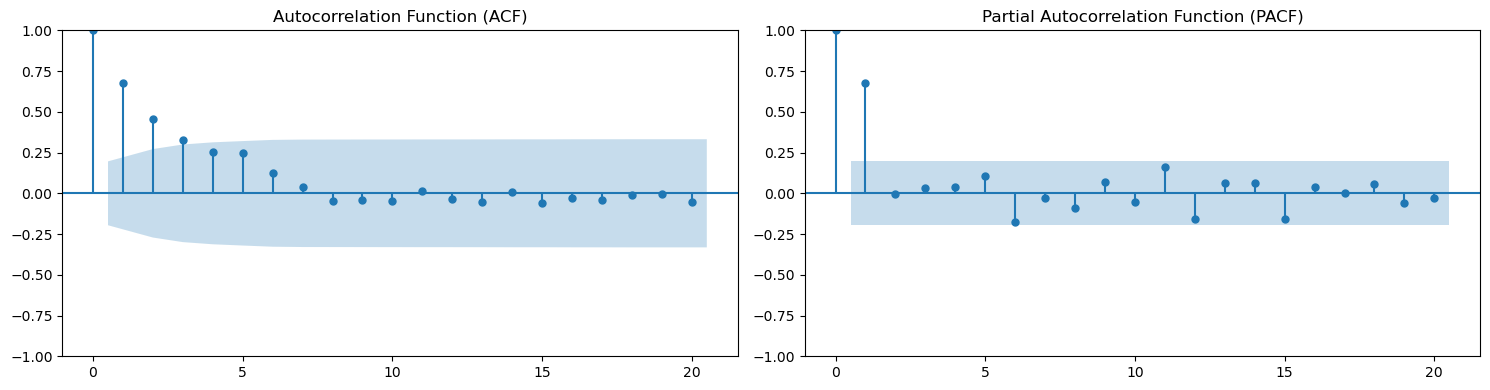
\includegraphics[width=0.8\linewidth]{images/acf-pacf.png}
	    \caption{ACF cuts off at lag 3 and PACF cuts off at lag 1}
	    \label{fig:}
	\end{figure}
	
	\subsection{Autocorrelation Function (ACF)}
	
	ACF measures the correlation between a time series and its lagged values.
	
	\begin{align*}
	\text{ACF}(k) = \frac{\text{Cov}(X_t, X_{t-k})}{\text{Var}(X_t)}
	\end{align*}
	
	Properties:
	\begin{itemize}
	\item Values range between $-1$ and $1$
	\item Lag 0 has autocorrelation equal to 1
	\item Shows how past values affect the current value
	\end{itemize}
	
	
	
	
	Model identification:
	\begin{itemize}
	\item ACF cuts off after lag $q$ $\rightarrow$ MA($q$) process
	\item Gradual decay $\rightarrow$ AR process
	\end{itemize}
	
	
	\subsection{Partial Autocorrelation Function (PACF)}
	
	PACF measures the direct relationship between $y_t$ and $y_{t-k}$ after removing the effect of intermediate lags $(1,2,\dots,k-1)$.
	
	\begin{itemize}
	\item \textbf{Definition:} PACF at lag $k$ is the coefficient $\phi_{kk}$ in the regression:
	\begin{align*}
	y_t = \phi_{k1} y_{t-1} + \phi_{k2} y_{t-2} + \cdots + \phi_{kk} y_{t-k} + \epsilon_t
	\end{align*}
	
	\item \textbf{Thus,}
	\begin{align*}
	\text{PACF}(k) = \phi_{kk}
	\end{align*}
	
	\item \textbf{Computation:}
	\begin{itemize}
	    \item Fit an AR($k$) model and take the last coefficient
	    \item Or compute recursively using Yule-Walker equations
	\end{itemize}
	
	\item \textbf{Interpretation:}
	\begin{itemize}
	    \item Measures \textit{direct} dependence between observations
	    \item Removes indirect effects captured in ACF
	\end{itemize}
	
	\item \textbf{Model Identification:}
	\begin{itemize}
	    \item Sharp cutoff in PACF $\Rightarrow$ suggests AR($p$)
	\end{itemize}
	\end{itemize}
	
	
	\subsection{Model Selection using AIC and BIC}
	
	The orders $(p,q,P,Q)$ in ARIMA and seasonal ARIMA models are selected by comparing candidate models using information criteria. A finite grid of models is specified by restricting $p,q,P,Q$ to small integers. For each candidate model, parameters are estimated via maximum likelihood, and the corresponding AIC or BIC value is computed. The preferred model is the one that minimizes the chosen criterion:
	\begin{align*}
	(p,q,P,Q) = \arg\min \ \text{IC}(p,q,P,Q),
	\end{align*}
	where $\text{IC} \in {\text{AIC}, \text{BIC}}$. The differencing orders $(d,D)$ are typically determined beforehand to ensure stationarity.
	
	The construction of AIC and BIC relies on the likelihood function. Consider a general time series model written as:
	\begin{align*}
	X_t = \hat{X}_t + \epsilon_t,
	\end{align*}
	where $\hat{X}_t$ is the fitted value and $\epsilon_t$ is the error term. It is assumed that:
	\begin{align*}
	\epsilon_t \sim \mathcal{N}(0,\sigma^2), \quad \text{i.i.d.}
	\end{align*}
	
	The likelihood of a single observation is given by the Gaussian density:
	\begin{align*}
	f(\epsilon_t) = \frac{1}{\sqrt{2\pi\sigma^2}} \exp\left(-\frac{\epsilon_t^2}{2\sigma^2}\right).
	\end{align*}
	
	Assuming independence, the likelihood of the entire series is:
	\begin{align*}
	L = \prod_{t=1}^{n} f(\epsilon_t)
	= \prod_{t=1}^{n} \frac{1}{\sqrt{2\pi\sigma^2}} \exp\left(-\frac{\epsilon_t^2}{2\sigma^2}\right).
	\end{align*}
	
	Taking logarithms, the log-likelihood becomes:
	\begin{align*}
	\log L
	&= -\frac{n}{2}\log(2\pi\sigma^2) - \frac{1}{2\sigma^2}\sum_{t=1}^{n} \epsilon_t^2.
	\end{align*}
	
	Maximizing this with respect to $\sigma^2$ yields:
	\begin{align*}
	\hat{\sigma}^2 = \frac{1}{n} \sum_{t=1}^{n} \epsilon_t^2,
	\end{align*}
	which shows that the likelihood depends directly on the sum of squared residuals. Substituting $\hat{\sigma}^2$ into the log-likelihood gives:
	\begin{align*}
	\log L = -\frac{n}{2}\log(2\pi) - \frac{n}{2}\log(\hat{\sigma}^2) - \frac{n}{2}.
	\end{align*}
	
	The information criteria are defined as:
	
	\begin{align*}
	AIC &= -2 \log L + 2k \\
	BIC &= -2 \log L + k \log n
	\end{align*}
	
	where $k$ is the number of estimated parameters. Substituting the log-likelihood expression:
	
	\begin{align*}
	AIC &= n \log(\hat{\sigma}^2) + 2k + \text{constant}, \\
	BIC &= n \log(\hat{\sigma}^2) + k \log n + \text{constant}
	\end{align*}
	
	
	Thus, both criteria depend on the residual variance (fit) and a penalty term (complexity). The optimal model minimizes this trade-off, balancing goodness of fit against over-parameterization.
	
	\paragraph{Maximization with respect to $\sigma^2$.}
	Treat the log-likelihood as a function of $\sigma^2$ with residuals ${\epsilon_t}$ fixed. Differentiating,
	\begin{align*}
	\frac{\partial}{\partial \sigma^2} \log L
	= -\frac{n}{2\sigma^2} + \frac{1}{2(\sigma^2)^2} \sum_{t=1}^{n} \epsilon_t^2.
	\end{align*}
	Setting the derivative to zero and solving gives
	\begin{align*}
	-\frac{n}{2\sigma^2} + \frac{1}{2(\sigma^2)^2} \sum_{t=1}^{n} \epsilon_t^2 &= 0 \
	\Rightarrow ; n\sigma^2 = \sum_{t=1}^{n} \epsilon_t^2 \
	\Rightarrow ; \hat{\sigma}^2 = \frac{1}{n} \sum_{t=1}^{n} \epsilon_t^2.
	\end{align*}
	Thus, the maximum likelihood estimate of the innovation variance is the average squared residual. Substituting $\hat{\sigma}^2$ into the log-likelihood yields an expression that depends only on the residual sum of squares, which directly drives AIC and BIC.
	
	
	\subsection{Moving Average (MA) Model}
	\paragraph{Introduction}
	A Moving Average (MA) model expresses a time series as a linear combination of current and past random shocks. The simplest form is the MA$(q)$ process:
	\begin{align*}
	\large X_t = \mu + \epsilon_t + \theta_1 \epsilon_{t-1} + \theta_2 \epsilon_{t-2} + \cdots + \theta_q \epsilon_{t-q}
	\end{align*}
	where ${\epsilon_t}$ is a white noise process with $\epsilon_t \sim \mathcal{N}(0,\sigma^2)$, and $\theta_1,\dots,\theta_q$ are parameters.
	
	The key idea is that the series is driven directly by shocks (innovations), and past shocks influence the current value only up to lag $q$. Unlike autoregressive models, the dependence is not on past values of $X_t$, but on past errors.
	
	For example, an MA$(1)$ model is:
	\begin{align*}
	\large X_t = \mu + \epsilon_t + \theta \epsilon_{t-1}
	\end{align*}
	
	\textit{Intuition.} A shock $\epsilon_t$ affects the series immediately and, through $\theta$, also affects the next period. However, after one lag, its effect disappears. Thus, shocks have \textit{temporary effects}, in contrast to unit root processes where shocks persist indefinitely.
	
	\paragraph{Mean and Variance of MA(q)} 
	Taking expectations:
	\begin{align*}
	\large \mathbb{E}[X_t] = \mu
	\end{align*}
	Since the $\epsilon_t$ are uncorrelated:
	\begin{align*}
	\large Var(X_t) = \sigma^2 (1 + \theta_1^2 + \cdots + \theta_q^2)
	\end{align*}
	Thus, the MA process is always stationary for any finite $q$.
	
	\paragraph{Autocovariance and Autocorrelation for MA$(1)$.}
	
	Consider the MA$(1)$ process:
	\begin{align*}
	X_t = \epsilon_t + \theta \epsilon_{t-1},
	\end{align*}
	where ${\epsilon_t}$ is white noise with $\mathbb{E}[\epsilon_t]=0$, $\text{Var}(\epsilon_t)=\sigma^2$, and $\text{Cov}(\epsilon_t,\epsilon_s)=0$ for $t \ne s$.
	
	The autocovariance at lag $h$ is defined as:
	\begin{align*}
	\gamma(h) = \text{Cov}(X_t, X_{t-h}).
	\end{align*}
	
	Variance ($h=0$):
	\begin{align*}
	\gamma(0) &= \text{Var}(X_t) \\
	&= \text{Var}(\epsilon_t + \theta \epsilon_{t-1}) \\
	&= \text{Var}(\epsilon_t) + \theta^2 \text{Var}(\epsilon_{t-1}) \\
	&= \sigma^2 + \theta^2 \sigma^2 \\
	&= \sigma^2(1+\theta^2),
	\end{align*}
	where cross terms vanish due to independence.
	
	Lag 1 ($h=1$):
	\begin{align*}
	\gamma(1) &= \text{Cov}(X_t, X_{t-1}) \\
	&= \text{Cov}(\epsilon_t + \theta \epsilon_{t-1}, \ \epsilon_{t-1} + \theta \epsilon_{t-2}) \\
	&= \text{Cov}(\epsilon_t, \epsilon_{t-1}) + \theta\,\text{Cov}(\epsilon_t, \epsilon_{t-2}) + \theta\,\text{Cov}(\epsilon_{t-1}, \epsilon_{t-1}) + \theta^2\,\text{Cov}(\epsilon_{t-1}, \epsilon_{t-2}),
	\end{align*}
	
	\begin{align*}
	\mathrm{Cov}(aX + bY,\, cZ + dW) = ac\,\mathrm{Cov}(X,Z) + ad\,\mathrm{Cov}(X,W) + bc\,\mathrm{Cov}(Y,Z) + bd\,\mathrm{Cov}(Y,W)
	\end{align*}
	
	
	
	Using white noise properties:
	\begin{align*}
	\text{Cov}(\epsilon_t, \epsilon_{t-1}) &= 0, \\
	\text{Cov}(\epsilon_t, \epsilon_{t-2}) &= 0, \\
	\text{Cov}(\epsilon_{t-1}, \epsilon_{t-2}) &= 0, \\
	\text{Cov}(\epsilon_{t-1}, \epsilon_{t-1}) &= \sigma^2,
	\end{align*}
	we obtain:
	\begin{align*}
	\large \gamma(1) = \theta \sigma^2
	\end{align*}
	
	
	Higher lags ($|h|>1$):
	\begin{align*}
	\large \gamma(h) = 0 \quad \text{for } |h| > 1
	\end{align*}
	because $X_t$ and $X_{t-h}$ do not share any common shock terms.
	
	
	The autocorrelation is:
	\begin{align*}
	\rho(h) = \frac{\gamma(h)}{\gamma(0)}.
	\end{align*}
	Thus,
	\begin{align*}
	\large \rho(1) = \frac{\theta \sigma^2}{\sigma^2(1+\theta^2)} = \frac{\theta}{1+\theta^2},
	\quad \rho(h)=0 \text{ for } |h|>1
	\end{align*}
	
	\textit{Key insight.} The autocovariance is nonzero only when $X_t$ and $X_{t-h}$ share common shock terms. In an MA$(1)$ process, shocks affect the series for only one lag, hence the autocorrelation function cuts off after lag 1. More generally, for an MA$(q)$ process, the ACF cuts off after lag $q$.
	
	\paragraph{Autocorrelation and Autocovariance for MA(q) Process}
	(Optional)
	
	
	Consider a moving average process of order $q$:
	\[
	X_t = \varepsilon_t + \theta_1 \varepsilon_{t-1} + \theta_2 \varepsilon_{t-2} + \cdots + \theta_q \varepsilon_{t-q}
	\]
	where $\{\varepsilon_t\}$ is white noise with $E[\varepsilon_t]=0$ and $\mathrm{Var}(\varepsilon_t)=\sigma^2$. Define $\theta_0 = 1$ for convenience, so that:
	\[
	X_t = \sum_{j=0}^{q} \theta_j \varepsilon_{t-j}.
	\]
	
	The autocovariance function at lag $h$ is:
	\[
	\gamma(h) = \mathrm{Cov}(X_t, X_{t-h}) = E[X_t X_{t-h}],
	\]
	since the mean is zero. Expanding both terms:
	\[
	X_t = \sum_{j=0}^{q} \theta_j \varepsilon_{t-j}, \quad
	X_{t-h} = \sum_{k=0}^{q} \theta_k \varepsilon_{t-h-k}.
	\]
	Hence,
	\[
	\gamma(h) = E\left[\left(\sum_{j=0}^{q} \theta_j \varepsilon_{t-j}\right)
	\left(\sum_{k=0}^{q} \theta_k \varepsilon_{t-h-k}\right)\right]
	= \sum_{j=0}^{q} \sum_{k=0}^{q} \theta_j \theta_k \, E[\varepsilon_{t-j}\varepsilon_{t-h-k}].
	\]
	
	Using the white noise property,
	\[
	E[\varepsilon_{t-j}\varepsilon_{t-h-k}] =
	\begin{cases}
	\sigma^2 & \text{if } j = h + k, \\
	0 & \text{otherwise},
	\end{cases}
	\]
	only terms with $j = h + k$ contribute. Therefore,
	\[
	\gamma(h) = \sigma^2 \sum_{k=0}^{q} \theta_{h+k}\theta_k.
	\]
	To ensure indices do not exceed $q$, we require $h+k \le q$, giving:
	
	\begin{align*}
	\large \gamma(h) = \sigma^2 \sum_{k=0}^{q-h} \theta_k \theta_{k+h}, \quad h \ge 0
	\end{align*}
	
	In particular,
	\[
	\gamma(0) = \sigma^2 \sum_{k=0}^{q} \theta_k^2,
	\]
	and for $h > q$, there are no valid terms, so $\gamma(h)=0$. Thus the autocovariance function truncates after lag $q$.
	
	The autocorrelation function is:
	
	\begin{align*}
	\large \rho(h) = \frac{\gamma(h)}{\gamma(0)} =
	\frac{\sum_{k=0}^{q-h} \theta_k \theta_{k+h}}{\sum_{k=0}^{q} \theta_k^2}, \quad 0 \le h \le q,
	\rho(h)=0 \quad \text{for } h>q
	\end{align*}
	
	The result shows that correlation arises only from overlapping noise terms in $X_t$ and $X_{t-h}$; beyond lag $q$, there is no overlap, which explains the sharp cutoff in the autocorrelation function.
	
	\paragraph{Invertibility and AR($\infty$) Representation.}
	
	For uniqueness of the MA representation, we impose the invertibility condition. For an MA$(1)$ process:
	\begin{align*}
	X_t = \epsilon_t + \theta \epsilon_{t-1},
	\end{align*}
	invertibility requires:
	\begin{align*}
	|\theta| < 1.
	\end{align*}
	
	
	Invertibility means that the unobserved shocks $\epsilon_t$ can be expressed in terms of past observed values $X_t$.
	
	
	Starting from:
	\begin{align*}
	X_t = \epsilon_t + \theta \epsilon_{t-1},
	\end{align*}
	\begin{align*}
	\epsilon_t = X_t - \theta \epsilon_{t-1}.
	\end{align*}
	
	Substitute the recursive expression for $\epsilon_{t-1}$ into the original model:
	\begin{align*}
	X_t &= \epsilon_t + \theta \epsilon_{t-1} \\
	&= \epsilon_t + \theta (X_{t-1} - \theta \epsilon_{t-2}) \\
	&= \epsilon_t + \theta X_{t-1} - \theta^2 \epsilon_{t-2}.
	\end{align*}
	
	Continue substituting:
	\begin{align*}
	X_t 
	&= \epsilon_t + \theta X_{t-1} - \theta^2 (X_{t-2} - \theta \epsilon_{t-3}) \\
	&= \epsilon_t + \theta X_{t-1} - \theta^2 X_{t-2} + \theta^3 \epsilon_{t-3} \\
	&\;\;\vdots \\
	&= \epsilon_t + \theta X_{t-1} - \theta^2 X_{t-2} + \theta^3 X_{t-3} - \cdots.
	\end{align*}
	
	Thus,
	\begin{align*}
	\large X_t = \epsilon_t + \sum_{i=1}^{\infty} (-\theta)^i X_{t-i}
	\end{align*}
	This infinite series converges only if $|\theta| < 1$.
	
	\textit{Key insight.} Under the invertibility condition $|\theta|<1$, the MA$(1)$ process can be expressed as an AR($\infty$) process with geometrically decaying coefficients.
	
	
	\textit{Intuition.}
	\begin{itemize}
	\item The original model depends on past \textit{shocks}.
	\item Invertibility allows us to express those shocks using past \textit{observations}.
	\item Thus, the process can be viewed as depending on infinitely many past values with diminishing weights.
	\end{itemize}
	
	\textit{Estimation.} Parameters are typically estimated via maximum likelihood. Unlike AR models, the likelihood is more complex because past errors are unobserved and must be inferred recursively.
	
	\paragraph{Why MA Models Do Not Have Closed-Form Solutions}
	
	\textit{AR vs MA Structure}:
	\[
	\text{AR(p): } X_t = \phi_1 X_{t-1} + \dots + \phi_p X_{t-p} + \epsilon_t
	\quad \Rightarrow \text{depends on observable past values}
	\]
	\[
	\text{MA(q): } X_t = \epsilon_t + \theta_1 \epsilon_{t-1} + \dots + \theta_q \epsilon_{t-q}
	\quad \Rightarrow \text{depends on unobserved past errors}
	\]
	
	\textit{Error Propagation in MA(1):}
	\[
	X_t = \epsilon_t + \theta \epsilon_{t-1} 
	\quad \Rightarrow \quad 
	\epsilon_t = X_t - \theta \epsilon_{t-1} 
	= X_t - \theta X_{t-1} + \theta^2 X_{t-2} - \theta^3 X_{t-3} + \dots
	\]
	\textit{(infinite backward chain in errors)}
	
	\textit{Contrast in Estimation:}
	\begin{itemize}
	    \item AR: finite recursion in observed $X$ → closed-form solution possible.
	    \[
	    \epsilon_t = X_t - \sum_{i=1}^{p} \phi_i X_{t-i} \quad (\text{finite})
	    \]
	    \item MA: infinite recursion in unobserved $\epsilon$ → closed-form solution impossible.
	    \[
	    \epsilon_t = X_t - \sum_{i=1}^{q} \theta_i \epsilon_{t-i} = X_t - \theta X_{t-1} + \theta^2 X_{t-2} - \dots \quad (\text{infinite})
	    \]
	\end{itemize}
	
	\textit{Conclusion:} 
	MA models depend on unobserved past errors that propagate infinitely. Therefore, we cannot express $\theta_i$ in closed form; numerical methods (e.g., iterative maximum likelihood) are required.
	
	
	\subsection{Autoregressive (AR) Model}
	An Autoregressive (AR) model expresses a time series as a linear function of its own past values. The simplest form is the AR$(p)$ process:
	\begin{align*}
	X_t = \mu + \phi_1 X_{t-1} + \phi_2 X_{t-2} + \cdots + \phi_p X_{t-p} + \epsilon_t
	\end{align*}
	where $\{\epsilon_t\}$ is a white noise process with $\epsilon_t \sim \mathcal{N}(0,\sigma^2)$, and $\phi_1,\dots,\phi_p$ are parameters.
	
	The key idea is that the current value of the series depends directly on its past values, with the noise term $\epsilon_t$ introducing new randomness at each time step.
	
	For example, an AR$(1)$ model is:
	\begin{align*}
	\large X_t = \mu + \phi X_{t-1} + \epsilon_t
	\end{align*}
	
	\textit{Intuition.} A shock $\epsilon_t$ affects the series immediately, but also propagates into the future through the dependence on past values. Thus, shocks have \textit{persistent effects}, in contrast to MA processes where effects are temporary.
	
	\paragraph{Mean and Stationarity.} Taking expectations:
	\begin{align*}
	\mathbb{E}[X_t] = \mu + \phi_1 \mathbb{E}[X_{t-1}] + \cdots + \phi_p \mathbb{E}[X_{t-p}].
	\end{align*}
	For a stationary process, $\mathbb{E}[X_t] = \mu_X$ is constant, giving:
	\begin{align*}
	\large \mu_X = \frac{\mu}{1 - \phi_1 - \cdots - \phi_p}
	\end{align*}
	provided the denominator is nonzero.
	
	\paragraph{Characteristic Equation for AR Models}
	Consider a general AR($p$) model:
	\begin{align*}
	X_t = \phi_1 X_{t-1} + \phi_2 X_{t-2} + \cdots + \phi_p X_{t-p} + \epsilon_t,
	\end{align*}
	where
	\begin{itemize}
	    \item $X_t$ is the time series at time $t$,
	    \item $\phi_1, \dots, \phi_p$ are autoregressive parameters,
	    \item $\epsilon_t$ is white noise with $\mathbb{E}[\epsilon_t] = 0$, $\text{Var}(\epsilon_t) = \sigma^2$, and $\text{Cov}(\epsilon_t,\epsilon_s)=0$ for $t \neq s$.
	\end{itemize}
	
	\textit{Move all $X$ terms to one side.}
	\begin{align*}
	X_t - \phi_1 X_{t-1} - \phi_2 X_{t-2} - \cdots - \phi_p X_{t-p} = \epsilon_t
	\end{align*}
	
	\textit{Express using the lag operator $L$} (where $L X_t = X_{t-1}$, $L^2 X_t = X_{t-2}$, etc.):
	\begin{align*}
	(1 - \phi_1 L - \phi_2 L^2 - \cdots - \phi_p L^p) X_t = \epsilon_t
	\end{align*}
	The polynomial
	\begin{align*}
	\large \phi(L) = 1 - \phi_1 L - \cdots - \phi_p L^p
	\end{align*}
	is called the AR polynomial.
	
	\textit{Consider the system without noise.}  
	To study intrinsic behavior (stability), set $\epsilon_t = 0$:
	\begin{align*}
	X_t - \phi_1 X_{t-1} - \cdots - \phi_p X_{t-p} = 0
	\end{align*}
	
	\textit{Try an exponential solution.}  
	Assume a solution of the form:
	\begin{align*}
	X_t = r^t
	\end{align*}
	where $r$ is a complex number. Substituting into the homogeneous equation:
	\begin{align*}
	r^t - \phi_1 r^{t-1} - \phi_2 r^{t-2} - \cdots - \phi_p r^{t-p} = 0
	\end{align*}
	Divide through by $r^{t-p}$:
	\begin{align*}
	\large r^p - \phi_1 r^{p-1} - \cdots - \phi_p = 0
	\end{align*}
	This is the characteristic equation of the AR($p$) process.
	
	\textit{Intuition:}  
	- The characteristic equation tells us how the system behaves without noise.  
	- The root $r$ determines whether shocks:
	\begin{itemize}
	    \item die out over time (stationary),
	    \item or persist/explode (non-stationary).
	\end{itemize}
	- This is exactly like solving linear differential equations, but in discrete time.
	
	
	\textit{Step 5: Stationarity condition.}  
	Let the roots of the characteristic equation be $r_1, r_2, \dots, r_p$.  
	The general solution of the homogeneous equation is:
	\begin{align*}
	X_t = C_1 r_1^t + C_2 r_2^t + \cdots + C_p r_p^t
	\end{align*}
	where $C_1,\dots,C_p$ are constants determined by initial conditions.
	
	- If $|r_i| < 1$ for all $i$, the terms decay over time → stationary process.
	- If any $|r_i| \ge 1$, the terms persist or explode → non-stationary.
	
	\textit{Example: AR(1) Characteristic Equation}
	
	Consider the AR(1) process:
	\begin{align*}
	X_t = \phi X_{t-1} + \epsilon_t,
	\end{align*}
	where
	\begin{itemize}
	    \item $X_t$ is the time series at time $t$,
	    \item $\phi$ is the autoregressive coefficient,
	    \item $\epsilon_t$ is white noise with mean $0$ and variance $\sigma^2$.
	\end{itemize}
	
	Write the characteristic equation using the general formula for AR($p$):
	\begin{align*}
	r^p - \phi_1 r^{p-1} - \cdots - \phi_p = 0.
	\end{align*}
	
	For AR(1), $p=1$ and $\phi_1 = \phi$
	\begin{align*}
	r - \phi = 0.
	\end{align*}
	
	
	The AR(1) process is stationary if the magnitude of the root is less than 1:
	\begin{align*}
	|r| < 1 \quad \Rightarrow \quad |\phi| < 1.
	\end{align*}
	
	
	\paragraph{Variance for AR$(1)$.} Consider:
	\begin{align*}
	X_t = \phi X_{t-1} + \epsilon_t,
	\end{align*}
	with zero mean. Then:
	\begin{align*}
	\text{Var}(X_t) &= \phi^2 \text{Var}(X_{t-1}) + \sigma^2.
	\end{align*}
	Under stationarity:
	\begin{align*}
	\large \gamma(0) = \frac{\sigma^2}{1 - \phi^2}
	\end{align*}
	
	\paragraph{Autocovariance and Autocorrelation of an AR(1) Process}
	
	
	Consider the autoregressive process of order 1:
	\[
	X_t = c + \phi X_{t-1} + \epsilon_t,
	\]
	where \(\{\epsilon_t\}\) is white noise with
	\[
	E[\epsilon_t] = 0, \quad \mathrm{Var}(\epsilon_t) = \sigma^2,
	\]
	and \(\epsilon_t\) is uncorrelated with past values \(X_{t-k}\), \(k \geq 1\).
	
	Assume \(|\phi| < 1\) so that the process is stationary.
	
	\textit{Mean of the Process}
	
	Taking expectation on both sides:
	\[
	E[X_t] = c + \phi E[X_{t-1}]
	\]
	
	Let \(E[X_t] = \mu\). Then:
	\[
	\mu = c + \phi \mu
	\Rightarrow \mu(1 - \phi) = c
	\]
	
	Hence:
	\[
	\mu = \frac{c}{1 - \phi}
	\]
	
	
	
	Define the centered process:
	\[
	Y_t = X_t - \mu
	\]
	
	Then:
	\begin{align*}
	Y_t &= X_t - \mu \\
	    &= (c + \phi X_{t-1} + \epsilon_t) - \mu \\
	    &= \phi (X_{t-1} - \mu) + \epsilon_t + (c - \mu)
	\end{align*}
	
	Using \(\mu = \frac{c}{1 - \phi}\), we get:
	\[
	c - \mu = -\phi \mu
	\]
	
	Thus:
	\[
	Y_t = \phi Y_{t-1} + \epsilon_t
	\]
	
	Hence, the centered process follows a zero-mean AR(1) model.
	
	\paragraph{Autocovariance Function}
	
	Define the autocovariance:
	\[
	\gamma(h) = \mathrm{Cov}(X_t, X_{t-h})
	\]
	
	Since covariance is invariant under shifts:
	\[
	\gamma(h) = \mathrm{Cov}(Y_t, Y_{t-h})
	\]
	
	For \(h \geq 1\):
	\begin{align*}
	\gamma(h) &= E[Y_t Y_{t-h}] \\
	          &= E[(\phi Y_{t-1} + \epsilon_t) Y_{t-h}] \\
	          &= \phi E[Y_{t-1} Y_{t-h}] + E[\epsilon_t Y_{t-h}]
	\end{align*}
	
	Since \(\epsilon_t\) is uncorrelated with past values:
	\[
	E[\epsilon_t Y_{t-h}] = 0
	\]
	
	Thus:
	\[
	\gamma(h) = \phi E[Y_{t-1} Y_{t-h}] = \phi \gamma(h-1)
	\]
	
	By repeated substitution:
	\[
	\gamma(h) = \phi \gamma(h-1) = \phi^2 \gamma(h-2) = \cdots = \phi^h \gamma(0)
	\]
	
	Hence:
	\[
	\gamma(h) = \phi^h \gamma(0)
	\]
	
	\paragraph{Autocorrelation Function}
	
	The autocorrelation function is defined as:
	\[
	\rho(h) = \frac{\gamma(h)}{\gamma(0)}
	\]
	
	Therefore:
	\[
	\rho(h) = \phi^h
	\]
	
	
	\textit{Key insight.} The autocorrelation function decays \textit{geometrically} rather than cutting off. This is the defining feature of AR processes.
	
	\paragraph{Yule--Walker Equations}
	
	Consider a stationary AR($p$) process:
	\[
	X_t = \phi_1 X_{t-1} + \phi_2 X_{t-2} + \cdots + \phi_p X_{t-p} + \epsilon_t,
	\]
	where \(E[\epsilon_t] = 0\), \(\mathrm{Var}(\epsilon_t) = \sigma^2\), and \(\epsilon_t\) is uncorrelated with \(X_{t-k}\) for all \(k \geq 1\). Assume \(E[X_t] = 0\).
	
	Recall the identity for any random variable \(Y\):
	\[
	\mathrm{Var}(Y) = E[Y^2] - (E[Y])^2.
	\]
	Hence, if \(E[Y] = 0\), then
	\[
	\mathrm{Var}(Y) = E[Y^2].
	\]
	In particular, since \(E[\epsilon_t] = 0\), we have
	\[
	E[\epsilon_t^2] = \sigma^2.
	\]
	
	Define the autocovariance function:
	\[
	\gamma(h) = \mathrm{Cov}(X_t, X_{t-h}) = E[X_t X_{t-h}].
	\]
	
	\medskip
	
	\textit{Row 0 (variance equation).}
	
	Multiply the model by \(X_t\) and take expectations:
	\begin{align*}
	\gamma(0) &= E[X_t^2] \\
	&= E\left[\left(\sum_{k=1}^p \phi_k X_{t-k} + \epsilon_t\right) X_t\right] \\
	&= \sum_{k=1}^p \phi_k E[X_{t-k} X_t] + E[\epsilon_t X_t].
	\end{align*}
	
	Now,
	\[
	E[\epsilon_t X_t]
	= E\left[\epsilon_t\left(\sum_{k=1}^p \phi_k X_{t-k} + \epsilon_t\right)\right]
	= \sum_{k=1}^p \phi_k E[\epsilon_t X_{t-k}] + E[\epsilon_t^2].
	\]
	Since \(\epsilon_t\) is uncorrelated with past values, \(E[\epsilon_t X_{t-k}] = 0\) for \(k \geq 1\). Therefore,
	\[
	E[\epsilon_t X_t] = E[\epsilon_t^2] = \sigma^2.
	\]
	
	Hence,
	\[
	\gamma(0) = \phi_1 \gamma(1) + \phi_2 \gamma(2) + \cdots + \phi_p \gamma(p) + \sigma^2
	\]
	
	\medskip
	
	\textit{Row 1.}
	
	Multiply the model by \(X_{t-1}\) and take expectations:
	\begin{align*}
	\gamma(1) &= E[X_t X_{t-1}] \\
	&= \sum_{k=1}^p \phi_k E[X_{t-k} X_{t-1}] + E[\epsilon_t X_{t-1}].
	\end{align*}
	
	Since \(E[\epsilon_t X_{t-1}] = 0\), we obtain:
	\[
	\gamma(1) = \phi_1 \gamma(0) + \phi_2 \gamma(1) + \cdots + \phi_p \gamma(p-1)
	\]
	
	\medskip
	
	\textit{Row 2.}
	
	Multiply the model by \(X_{t-2}\):
	\begin{align*}
	\gamma(2) &= E[X_t X_{t-2}] \\
	&= \sum_{k=1}^p \phi_k E[X_{t-k} X_{t-2}].
	\end{align*}
	
	Thus:
	\[
	\gamma(2) = \phi_1 \gamma(1) + \phi_2 \gamma(0) + \cdots + \phi_p \gamma(p-2)
	\]
	
	\medskip
	
	Continuing similarly, for general \(h \geq 1\):
	\[
	\gamma(h) = \phi_1 \gamma(h-1) + \phi_2 \gamma(h-2) + \cdots + \phi_p \gamma(h-p)
	\]
	
	\medskip
	
	Collecting the first \(p\) equations:
	\begin{align*}
	\gamma(1) &= \phi_1 \gamma(0) + \phi_2 \gamma(1) + \cdots + \phi_p \gamma(p-1), \\
	\gamma(2) &= \phi_1 \gamma(1) + \phi_2 \gamma(0) + \cdots + \phi_p \gamma(p-2), \\
	&\;\;\vdots \\
	\gamma(p) &= \phi_1 \gamma(p-1) + \phi_2 \gamma(p-2) + \cdots + \phi_p \gamma(0).
	\end{align*}
	
	\medskip
	
	These equations can be written in matrix form as:
	\[
	\begin{bmatrix}
	\gamma(0) & \gamma(1) & \cdots & \gamma(p-1) \\
	\gamma(1) & \gamma(0) & \cdots & \gamma(p-2) \\
	\vdots & \vdots & \ddots & \vdots \\
	\gamma(p-1) & \gamma(p-2) & \cdots & \gamma(0)
	\end{bmatrix}
	\begin{bmatrix}
	\phi_1 \\
	\phi_2 \\
	\vdots \\
	\phi_p
	\end{bmatrix}
	=
	\begin{bmatrix}
	\gamma(1) \\
	\gamma(2) \\
	\vdots \\
	\gamma(p)
	\end{bmatrix}.
	\]
	
	\medskip
	
	If the matrix is invertible, then
	\[
	\boldsymbol{\phi} = \Gamma^{-1} \boldsymbol{\gamma}
	\]
	
	
	\textit{General AR$(p)$ Process.}
	
	For:
	\begin{align*}
	X_t = \phi_1 X_{t-1} + \cdots + \phi_p X_{t-p} + \epsilon_t,
	\end{align*}
	the autocovariances satisfy the Yule--Walker equations:
	\begin{align*}
	\large \gamma(h) = \phi_1 \gamma(h-1) + \cdots + \phi_p \gamma(h-p), \quad h \geq 1
	\end{align*}
	
	\textit{Key insight.} Unlike MA processes, the ACF of an AR$(p)$ process does not cut off but instead decays gradually (often exponentially or in a damped sinusoidal pattern).
	
	\paragraph{Partial Autocorrelation Function (PACF).}
	
	The PACF measures the direct dependence between $X_t$ and $X_{t-h}$ after removing intermediate effects.
	
	\begin{itemize}
	\item For an AR$(p)$ process, the PACF cuts off after lag $p$.
	\item This provides a key identification tool for AR models.
	\end{itemize}
	
	\paragraph{Causal Representation (AR(1)= MA($\infty$) Form).}
	
	An AR$(1)$ process can be written as:
	\begin{align*}
	X_t &= \phi X_{t-1} + \epsilon_t\\
	X_{t-1} &= \phi X_{t-2} + \epsilon_{t-1}\\
	X_{t-2} &= \phi X_{t-3} + \epsilon_{t-2}
	\end{align*}
	
	
	Substituting recursively:
	\begin{align*}
	\large X_t = \sum_{i=0}^{\infty} \phi^i \epsilon_{t-i}
	\end{align*}
	
	This infinite series converges only if $|\phi| < 1$.
	
	\textit{Key insight.} Under the stationarity condition, the AR$(1)$ process can be expressed as an MA($\infty$) process with geometrically decaying weights.
	
	\textit{Interpretation.}
	\begin{itemize}
	\item The AR model depends on past \textit{values} of the series.
	\item The MA($\infty$) representation shows that it can also be viewed as depending on all past \textit{shocks}.
	\item The influence of shocks decays gradually over time.
	\end{itemize}
	
	
	
	\subsection{Autoregressive Moving Average (ARMA) Model}
	
	An Autoregressive Moving Average (ARMA) model combines the features of both AR and MA processes, allowing the series to depend on its past values as well as past shocks. An ARMA$(p,q)$ process is defined as:
	\[
	\large X_t = \phi_1 X_{t-1} + \cdots + \phi_p X_{t-p} + \epsilon_t + \theta_1 \epsilon_{t-1} + \cdots + \theta_q \epsilon_{t-q}
	\]
	
	where ${\epsilon_t}$ is white noise with $\epsilon_t \sim \mathcal{N}(0,\sigma^2)$.
	
	Using the backshift operator $B$, the model can be written compactly as:
	\begin{align*}
	\large \phi(B)X_t = \theta(B)\epsilon_t
	\end{align*}
	where
	\begin{align*}
	\phi(B) = 1 - \phi_1 B - \cdots - \phi_p B^p, \quad
	\theta(B) = 1 + \theta_1 B + \cdots + \theta_q B^q.
	\end{align*}
	
	\textit{Intuition.} The AR component captures persistence through past values, while the MA component captures the direct impact of past shocks. Thus, ARMA models provide a flexible framework where shocks both propagate over time (AR effect) and have short-term direct influence (MA effect).
	
	\textit{Causality and Invertibility.} For the ARMA process to be well-defined and uniquely represented:
	\begin{itemize}
	\item \textbf{Causality (Stationarity):} The roots of $\phi(z)=0$ must lie outside the unit circle. This ensures:
	\begin{align*}
	X_t = \frac{1}{\phi(B)}\theta(B)\epsilon_t = \sum_{j=0}^{\infty} \psi_j \epsilon_{t-j}.
	\end{align*}
	\item \textbf{Invertibility:} The roots of $\theta(z)=0$ must lie outside the unit circle. This ensures:
	\begin{align*}
	\epsilon_t = \frac{1}{\theta(B)}\phi(B)X_t = \sum_{j=0}^{\infty} \pi_j X_{t-j}.
	\end{align*}
	\end{itemize}
	
	\textit{AR($\infty$) and MA($\infty$) Representations.} Under these conditions, the ARMA process admits dual representations:
	\begin{align*}
	X_t &= \sum_{j=0}^{\infty} \psi_j \epsilon_{t-j} \quad \text{(MA($\infty$))}, \\
	X_t &= \sum_{j=1}^{\infty} \pi_j X_{t-j} + \epsilon_t \quad \text{(AR($\infty$))}.
	\end{align*}
	
	\textit{Example: ARMA$(1,1)$.}
	\begin{align*}
	X_t = \phi X_{t-1} + \epsilon_t + \theta \epsilon_{t-1}.
	\end{align*}
	Using the operator form:
	\begin{align*}
	(1 - \phi B)X_t = (1 + \theta B)\epsilon_t.
	\end{align*}
	If $|\phi|<1$, we can expand:
	\begin{align*}
	X_t = \frac{1+\theta B}{1-\phi B}\epsilon_t
	= (1+\theta B)\sum_{j=0}^{\infty} \phi^j B^j \epsilon_t,
	\end{align*}
	which yields an MA($\infty$) representation.
	
	
	\subsection{Autoregressive Integrated Moving Average (ARIMA) Model}
	
	An Autoregressive Integrated Moving Average (ARIMA) model extends ARMA models to handle non-stationary time series by introducing differencing. An ARIMA$(p,d,q)$ process assumes that the $d$-th differenced series is stationary and follows an ARMA$(p,q)$ model.
	
	Let the differencing operator be defined using the backshift operator $B$:
	\begin{align*}
	\Delta X_t = (1 - B)X_t, \quad \Delta^d X_t = (1 - B)^d X_t.
	\end{align*}
	
	Then an ARIMA$(p,d,q)$ model is given by:
	\begin{align*}
	\large \phi(B)(1 - B)^d X_t = \theta(B)\epsilon_t
	\end{align*}
	where:
	\begin{align*}
	\phi(B) &= 1 - \phi_1 B - \cdots - \phi_p B^p, \\
	\theta(B) &= 1 + \theta_1 B + \cdots + \theta_q B^q,
	\end{align*}
	and ${\epsilon_t}$ is white noise with $\epsilon_t \sim \mathcal{N}(0,\sigma^2)$.
	
	\textit{Intuition.} Many real-world time series exhibit trends or non-stationary behavior. Differencing removes these trends:
	\begin{itemize}
	\item $d=0$: already stationary (ARMA model),
	\item $d=1$: removes linear trend (random walk-type behavior),
	\item $d>1$: removes higher-order trends.
	\end{itemize}
	After differencing, the transformed series behaves like a stationary ARMA process.
	
	\textit{Example: ARIMA$(1,1,1)$.}
	\begin{align*}
	(1 - \phi B)(1 - B)X_t = (1 + \theta B)\epsilon_t.
	\end{align*}
	Expanding the differencing term:
	\begin{align*}
	(1 - B)X_t = X_t - X_{t-1},
	\end{align*}
	so the model effectively applies an ARMA structure to the first differences.
	
	\textit{Unit Root Interpretation.} The factor $(1 - B)^d$ introduces $d$ unit roots. For example:
	\begin{align*}
	(1 - B)X_t = \epsilon_t \quad \Rightarrow \quad X_t = X_{t-1} + \epsilon_t,
	\end{align*}
	which is a random walk (non-stationary). Thus, ARIMA models explicitly account for unit root behavior.
	
	\textit{Stationarity and Invertibility.} After differencing, the ARMA component must satisfy:
	\begin{itemize}
	\item Roots of $\phi(z)=0$ lie outside the unit circle (stationarity/causality),
	\item Roots of $\theta(z)=0$ lie outside the unit circle (invertibility).
	\end{itemize}
	
	\textit{Infinite Representations.} If the above conditions hold, the differenced process admits:
	\begin{align*}
	\Delta^d X_t = \sum_{j=0}^{\infty} \psi_j \epsilon_{t-j}.
	\end{align*}
	Thus, the original series can be viewed as a cumulative sum of past shocks.
	
	\textit{Key insight.} ARIMA models separate:
	\begin{itemize}
	\item \textbf{Non-stationarity} (handled by differencing),
	\item \textbf{Dependence structure} (captured by ARMA).
	\end{itemize}
	
	\textit{Estimation and Identification.} The typical workflow involves:
	\begin{itemize}
	\item Determining $d$ using unit root tests,
	\item Selecting $(p,q)$ using ACF/PACF and AIC/BIC,
	\item Estimating parameters via maximum likelihood.
	\end{itemize}
	
	\textit{Summary intuition.} An ARIMA model describes a process where:
	\begin{itemize}
	\item The series may be non-stationary in levels,
	\item Differencing transforms it into a stationary process,
	\item The stationary component follows an ARMA structure,
	\item The observed series is an accumulation of past shocks.
	\end{itemize}
	
	
	\subsection{Seasonal Autoregressive Integrated Moving Average (SARIMA)}
	
	A Seasonal ARIMA model extends ARIMA to capture periodic (seasonal) patterns in time series data. It incorporates both non-seasonal and seasonal dynamics.
	
	\begin{align*}
	\large y_t = c + \sum_{i=1}^{p} \phi_i y_{t-i} + \sum_{j=1}^{q} \theta_j \epsilon_{t-j} + \sum_{I=1}^{P} \Phi_I y_{t-Is} + \sum_{J=1}^{Q} \Theta_J \epsilon_{t-Js} + \epsilon_t
	\end{align*} 
	
	This equation is applied to a stationary (differenced) time series, not the original raw series.
	
	A \textbf{SARIMA$(p,d,q)(P,D,Q)_s$} model is defined as(Using Backshift operator):
	\begin{align*}
	\large \phi(B)\Phi(B^s)(1 - B)^d (1 - B^s)^D X_t = \theta(B)\Theta(B^s)\epsilon_t
	\end{align*}
	where:
	\begin{align*}
	\phi(B) &= 1 - \phi_1 B - \cdots - \phi_p B^p, \\
	\theta(B) &= 1 + \theta_1 B + \cdots + \theta_q B^q, \\
	\Phi(B^s) &= 1 - \Phi_1 B^s - \cdots - \Phi_P B^{Ps}, \\
	\Theta(B^s) &= 1 + \Theta_1 B^s + \cdots + \Theta_Q B^{Qs}.
	\end{align*}
	
	\textit{Components.}
	\begin{itemize}
	\item $(p,d,q)$ : non-seasonal AR, differencing, MA orders
	\item $(P,D,Q)$ : seasonal AR, differencing, MA orders
	\item $s$ : seasonal period (e.g., $s=12$ for monthly data)
	\end{itemize}
	
	\textit{Differencing.} Stationarity is achieved through:
	\begin{align*}
	(1 - B)^d &\quad \text{(non-seasonal differencing)},\\
	\quad (1 - B^s)^D &\quad \text{(seasonal differencing)}.
	\end{align*}
	For example:
	\begin{align*}
	(1 - B^s)X_t = X_t - X_{t-s},
	\end{align*}
	which removes seasonal patterns.
	
	\textit{Expanded form.} The model combines:
	\begin{itemize}
	\item Non-seasonal AR terms: dependence on recent lags
	\item Seasonal AR terms: dependence on values $s, 2s, \dots$ periods ago
	\item Non-seasonal MA terms: short-term shock effects
	\item Seasonal MA terms: seasonal shock effects
	\end{itemize}
	
	\textit{Intuition.}
	\begin{itemize}
	\item Non-seasonal components capture short-term dynamics.
	\item Seasonal components capture repeating patterns across seasons.
	\item Differencing removes trend and seasonality before modeling dependence.
	\end{itemize}
	
	\textit{Example: SARIMA$(1,1,1)(1,1,1)_s$.}
	\begin{align*}
	(1 - \phi B)(1 - \Phi B^s)(1 - B)(1 - B^s)X_t = (1 + \theta B)(1 + \Theta B^s)\epsilon_t.
	\end{align*}
	
	\textit{Stationarity and Invertibility.}
	\begin{itemize}
	\item Roots of $\phi(z)\Phi(z^s)=0$ must lie outside the unit circle (stationarity/causality).
	\item Roots of $\theta(z)\Theta(z^s)=0$ must lie outside the unit circle (invertibility).
	\end{itemize}
	
	\textit{Interpretation.}
	\begin{itemize}
	\item The original series may be non-stationary due to trend and seasonality.
	\item Differencing transforms it into a stationary series.
	\item The stationary component follows an ARMA structure with both seasonal and non-seasonal terms.
	\end{itemize}
	
	\textit{Conceptual view.}
	\begin{align*}
	\text{SARIMA} = \text{ARMA applied after removing trend and seasonality}.
	\end{align*}
	
	\textit{Summary intuition.}
	\begin{itemize}
	\item The series evolves through both short-term and seasonal dependencies.
	\item Shocks propagate locally (AR) and seasonally (SAR).
	\item Differencing ensures stability, while ARMA structure captures dependence.
	\end{itemize}
	
	
	
	\subsection{Identifying Seasonal Orders using ACF and PACF}
	
	To determine the appropriate seasonal orders for the SARIMA model, the following step-by-step procedure is illustrated through the sequence of plots:
	
	\begin{itemize}
	\item First, the ACF and PACF plots of the \textbf{first-order differenced series} are examined to assess stationarity and initial autocorrelation structure.
	
	\item The ACF plot reveals a \textbf{repeating pattern at regular intervals}, indicating the presence of seasonality in the data.
	
	\item To eliminate this seasonal pattern, \textbf{seasonal differencing} is applied with an appropriate seasonal period $s$.
	
	\item After seasonal differencing, the ACF and PACF plots are re-evaluated. The absence of repeating patterns confirms that the \textbf{seasonality has been effectively removed}.
	
	\item Finally, the lag structure is carefully analyzed by dividing the lags into \textbf{seasonal groups}, which helps in identifying the seasonal autoregressive ($P$) and seasonal moving average ($Q$) orders.
	
	\item Based on these observations, suitable values for the seasonal parameters $(P, D, Q)_s$ are selected.
	\end{itemize}
	
	\begin{figure}[H]
	    \centering
	    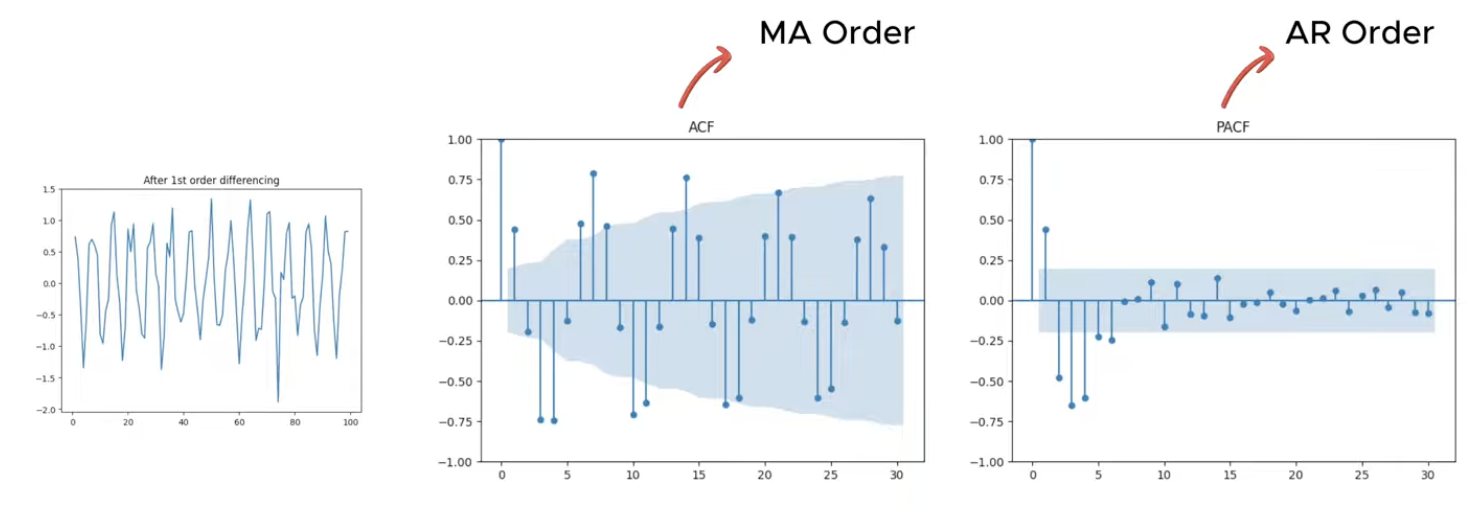
\includegraphics[width=0.8\linewidth]{images/4acf-pacf-after-first-order-differencing.png}
	    \caption{ACF-PACF Plots after the first order differencing(d=1)}
	    \label{fig:svm_main}
	\end{figure}
	\begin{figure}[H]
	    \centering
	    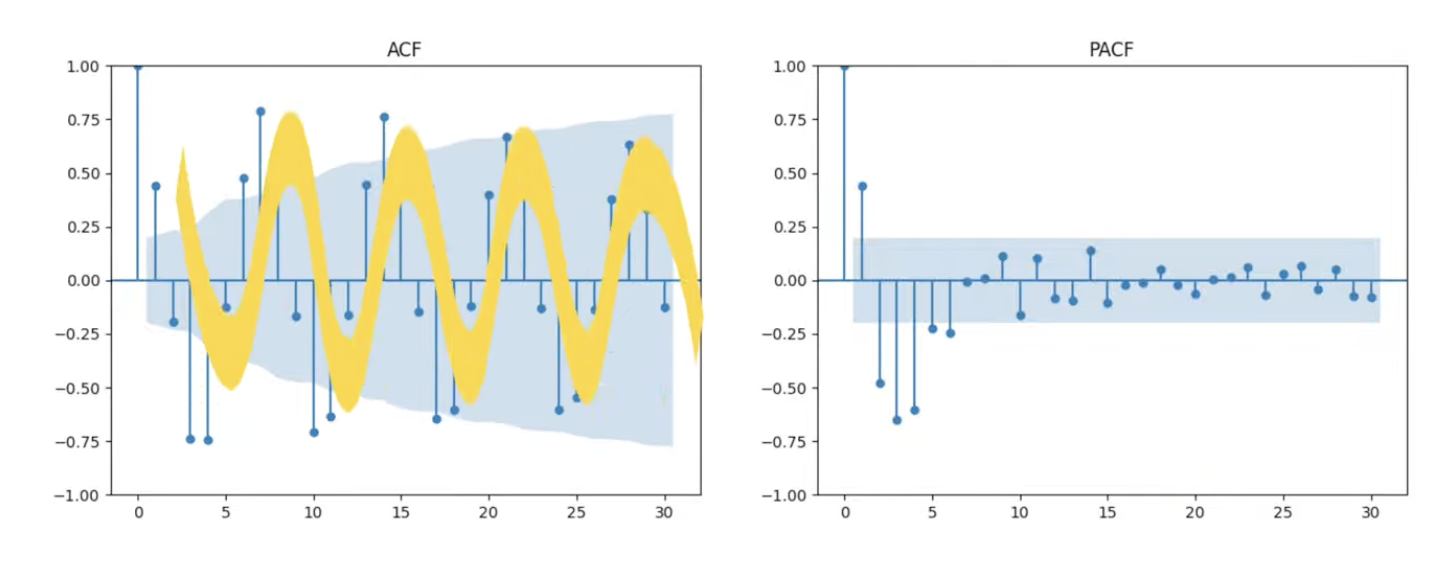
\includegraphics[width=0.8\linewidth]{images/5.patterns-in-acf.png}
	    \caption{We can see the patterns in the acf plots which suggests the need of seasonal differencing}
	    \label{fig:svm_main}
	\end{figure}
	\begin{figure}[H]
	    \centering
	    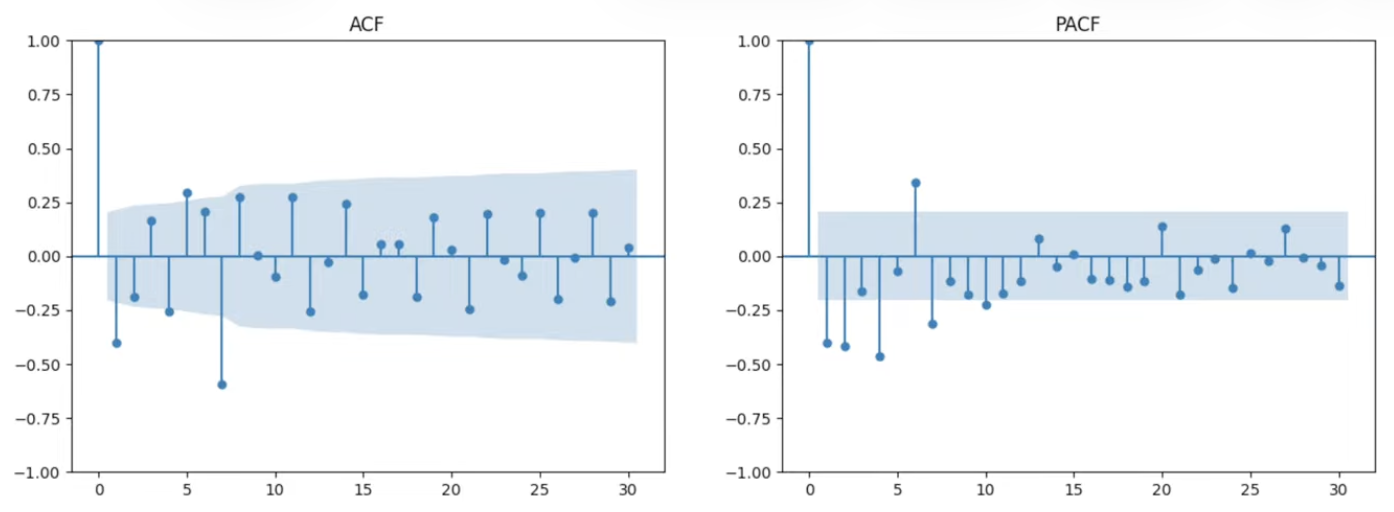
\includegraphics[width=0.8\linewidth]{images/6acf-pacf-after-seasonal-differencing.png}
	    \caption{ACF-PACF After the seasonal differencing}
	    \label{fig:svm_main}
	\end{figure}
	\begin{figure}[H]
	    \centering
	    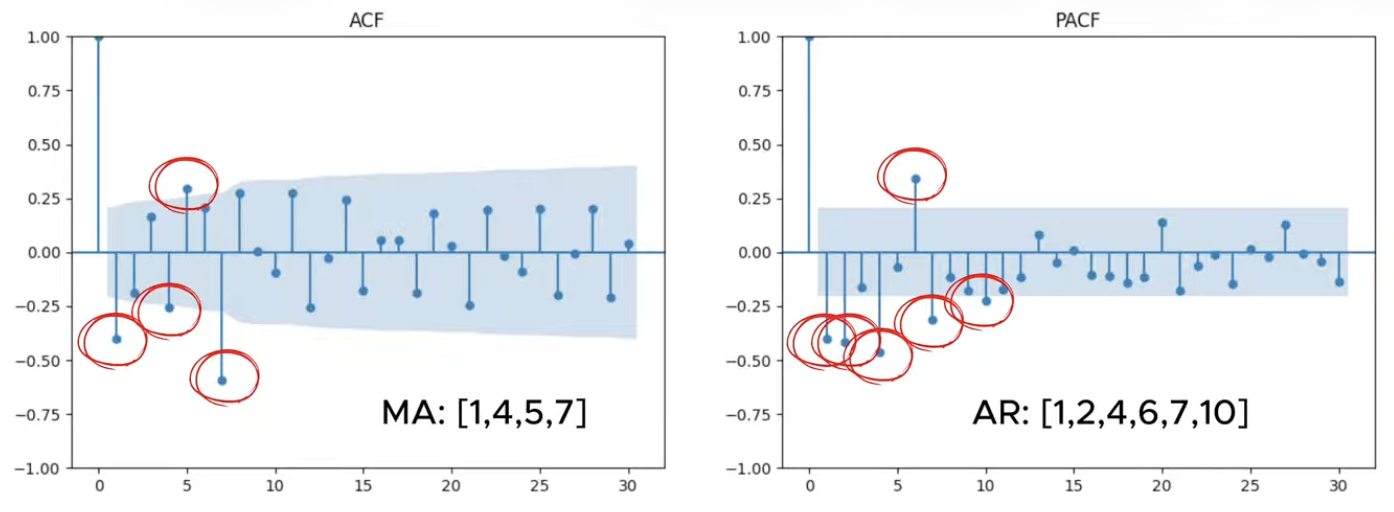
\includegraphics[width=0.8\linewidth]{images/7-ar-ma-possible-combinations.png}
	    \caption{Possible order combinations for AR/MA }
	    \label{fig:svm_main}
	\end{figure}
	
	\begin{figure}[H]
	    \centering
	    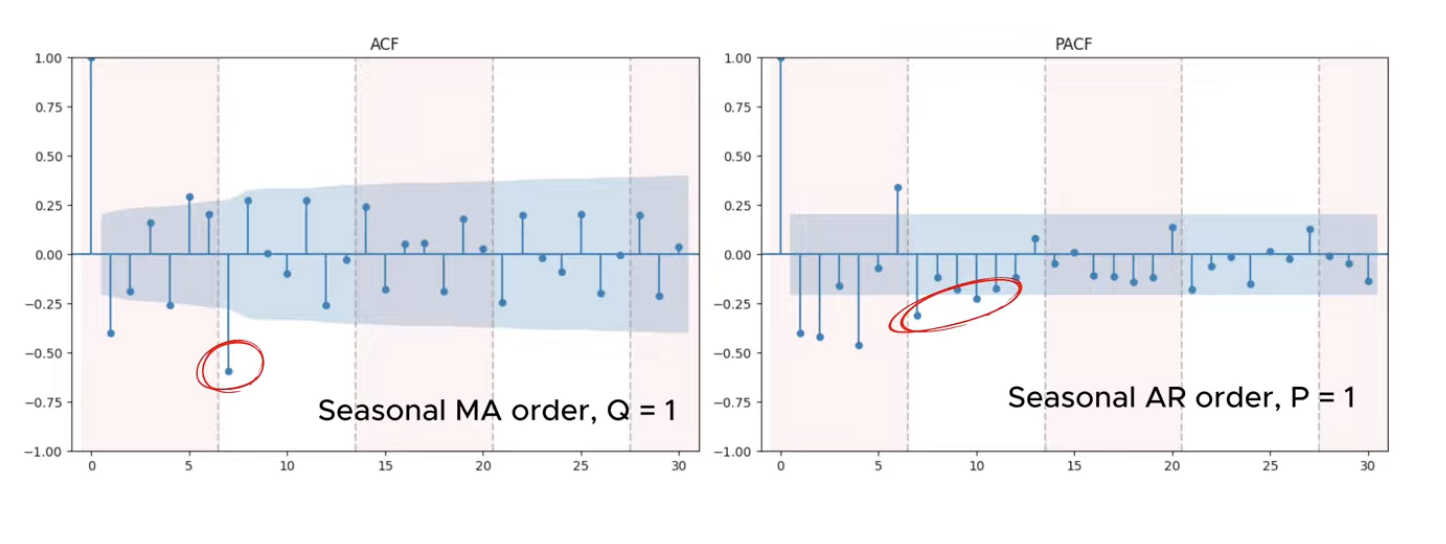
\includegraphics[width=0.8\linewidth]{images/8finding-sarima-orders.png}
	    \caption{Finding the seasonal orders}
	    \label{fig:svm_main}
	\end{figure}
	
	\subsection{Vector Autoregressive (VAR) and VARMA Models}
	
	In many real-world problems, multiple time series evolve together and influence each other. For example, economic variables such as inflation, interest rates, and GDP are interdependent. Modeling each series separately ignores these interactions. VAR and VARMA models are designed to capture such joint dynamics.
	
	A Vector Autoregressive model of order $p$, denoted VAR$(p)$, models a vector of time series $X_t \in \mathbb{R}^k$ as:
	\begin{align*}
	X_t = c + A_1 X_{t-1} + A_2 X_{t-2} + \cdots + A_p X_{t-p} + \epsilon_t,
	\end{align*}
	where $c$ is a constant vector, $A_i$ are coefficient matrices, and $\epsilon_t$ is a white noise vector.
	
	The key idea is simple: each variable depends not only on its own past values but also on the past values of all other variables in the system. This allows the model to capture feedback and interaction effects over time.
	
	For example, in a two-variable VAR(1) system:
	\begin{equation*}
	\begin{bmatrix} y_{1t} \\ y_{2t} \end{bmatrix}
	=
	\begin{bmatrix} c_1 \\ c_2 \end{bmatrix}
	+
	\begin{bmatrix} a_{11} & a_{12} \\ a_{21} & a_{22} \end{bmatrix}
	\begin{bmatrix} y_{1,t-1} \\ y_{2,t-1} \end{bmatrix}
	+
	\begin{bmatrix} \varepsilon_{1t} \\ \varepsilon_{2t} \end{bmatrix}.
	\end{equation*}
	
	Here, each variable is influenced by both its own lag and the lag of the other variable.
	
	We care about VAR models because they:
	\begin{itemize}
	\item capture interactions between multiple time series,
	\item are useful for forecasting systems of variables,
	\item help analyze how shocks to one variable affect others over time.
	\end{itemize}
	
	Estimation of VAR models is straightforward. Since each equation involves the same regressors (lagged variables), the system can be estimated equation-by-equation using ordinary least squares (OLS). This simplicity is one of the main advantages of VAR models.
	
	\vspace{0.5em}
	
	A Vector Autoregressive Moving Average model, VARMA$(p,q)$, extends VAR by including past shocks:
	\begin{align*}
	X_t = c + A_1 X_{t-1} + \cdots + A_p X_{t-p} + \epsilon_t + M_1 \epsilon_{t-1} + \cdots + M_q \epsilon_{t-q}.
	\end{align*}
	
	The additional moving average terms allow the model to capture how past shocks propagate through the system over time. While VAR focuses on dependence through past values, VARMA also accounts for the lingering effects of past disturbances.
	
	In practice:
	\begin{itemize}
	\item VAR models are more commonly used due to their simplicity and ease of estimation.
	\item VARMA models are more flexible but harder to estimate because past errors are unobserved.
	\end{itemize}
	
	\textit{Summary intuition.}
	\begin{itemize}
	\item VAR models describe how variables influence each other over time.
	\item VARMA models additionally capture how shocks spread across variables.
	\item Both provide a framework for understanding and forecasting multivariate time series.
	\end{itemize}
	
	
	\subsection{VAR Model Example}
	We consider two related time series: \textit{ice cream sales} and \textit{heater sales}, which are expected to exhibit opposite seasonal behavior. The objective is to model their dynamic relationship and understand how past values of each variable influence the other over time using a VAR model.
	\begin{itemize}
	\item Number of Equations: 2
	\item Number of Observations: 184
	\item Log Likelihood: -204.405
	\item AIC: -2.867
	\item BIC: -1.923
	\item HQIC: -2.485
	\item FPE: 0.0571
	\end{itemize}
	
	\paragraph{Results for equation: Ice Cream}
	
	\begin{center}
	\begin{tabular}{lrrrr}
	\toprule
	Variable & Coefficient & Std. Error & t-stat & p-value \\
	\midrule
	Const & -0.0161 & 0.0341 & -0.471 & 0.638 \\
	L1.Ice Cream & -0.2878 & 0.0796 & -3.614 & 0.000 \\
	L1.Heater & -0.1213 & 0.0737 & -1.646 & 0.100 \\
	L2.Ice Cream & -0.2179 & 0.0870 & -2.503 & 0.012 \\
	L2.Heater & -0.0820 & 0.0798 & -1.028 & 0.304 \\
	L3.Ice Cream & -0.1222 & 0.0908 & -1.346 & 0.178 \\
	L3.Heater & -0.1007 & 0.0807 & -1.248 & 0.212 \\
	L4.Ice Cream & -0.1675 & 0.0891 & -1.880 & 0.060 \\
	L4.Heater & -0.1305 & 0.0822 & -1.587 & 0.112 \\
	L5.Ice Cream & -0.2067 & 0.0903 & -2.288 & 0.022 \\
	L5.Heater & -0.1686 & 0.0850 & -1.984 & 0.047 \\
	\bottomrule
	\end{tabular}
	\end{center}
	
	\paragraph{Results for equation: Heater}
	\begin{center}
	\begin{tabular}{lrrrr}
	\toprule
	Variable & Coefficient & Std. Error & t-stat & p-value \\
	\midrule
	Const & 0.0059 & 0.0361 & 0.162 & 0.871 \\
	
	L1.Ice Cream & -0.0331 & 0.0842 & -0.393 & 0.694 \\
	\textbf{\color{red}L1.Heater} & \textbf{\color{red}-0.4054} & 0.0779 & -5.204 & \textbf{\color{red}0.000} \\
	
	L2.Ice Cream & -0.1698 & 0.0920 & -1.845 & 0.065 \\
	\textbf{\color{red}L2.Heater} & \textbf{\color{red}-0.1936} & 0.0844 & -2.294 & \textbf{\color{red}0.022} \\
	
	L3.Ice Cream & -0.0490 & 0.0960 & -0.511 & 0.610 \\
	L3.Heater & -0.0170 & 0.0854 & -0.199 & 0.843 \\
	
	L4.Ice Cream & -0.0076 & 0.0942 & -0.081 & 0.935 \\
	L4.Heater & 0.0095 & 0.0870 & 0.109 & 0.913 \\
	
	L5.Ice Cream & -0.0203 & 0.0955 & -0.212 & 0.832 \\
	L5.Heater & -0.0506 & 0.0899 & -0.563 & 0.573 \\
	
	\textbf{\color{red}L13.Ice Cream} & \textbf{\color{red}0.2035} & 0.0921 & 2.210 & \textbf{\color{red}0.027} \\
	
	\bottomrule
	\end{tabular}
	\end{center}
	
	
	\paragraph{Correlation Matrix of Residuals}
	
	\begin{center}
	\begin{tabular}{lcc}
	\toprule
	 & Ice Cream & Heater \\
	\midrule
	Ice Cream & 1.000 & 0.065 \\
	Heater    & 0.065 & 1.000 \\
	\bottomrule
	\end{tabular}
	\end{center}
	
	\paragraph{Interpretation}
	Since, our variable of interest is Heater ; the final model is (based on the significance)
	$$
	\hat{h}_t = - 0.41h_{t-1} - 0.19h_{t-2} + 0.2i_{t-13}
	$$
	
	The VAR model suggests that both variables depend on their own past values as well as the lagged values of the other variable. Significant coefficients at lower lags indicate strong short-term dynamics, while higher lags show weaker influence.
	
\end{document}